% =====================================================================
% ภาคผนวก ก ภาพหน้าจอของระบบ
% =====================================================================

ภาคผนวกนี้แสดงภาพหน้าจอส่วนติดต่อกับผู้ใช้ของระบบรวบรวมและสังเคราะห์ประเด็นข่าวภาษาไทยอัตโนมัติที่พัฒนาเสร็จสมบูรณ์แล้ว โดยข้อมูลและภาพประกอบที่แสดงเป็นผลลัพธ์จากการดึงและประมวลผลข่าวสารจริงในระบบ

\section{หน้าจอหลัก Bento Hub SPA}

หน้าจอหลักของระบบนำเสนอข่าวสารสดในรูปแบบ Bento Hub แบบ Single Page Application ซึ่งจัดวางองค์ประกอบข่าวแบบ Responsive Grid แสดงบัตรสรุปข่าวเด่น แถบเลือกหมวดหมู่ข่าว 9 หมวดหมู่ ปุ่มคัดกรองสำนักข่าว ช่องสืบค้นคำสำคัญ แถบแฮชแท็กประเด็นร้อน และแบนเนอร์แจ้งเตือนข่าวใหม่ลอยตัวที่อัปเดตแบบเรียลไทม์ ดังแสดงในภาพที่~\ref{fig_screenshot_bento}

\begin{figure}[H]
\centering
\imgframe{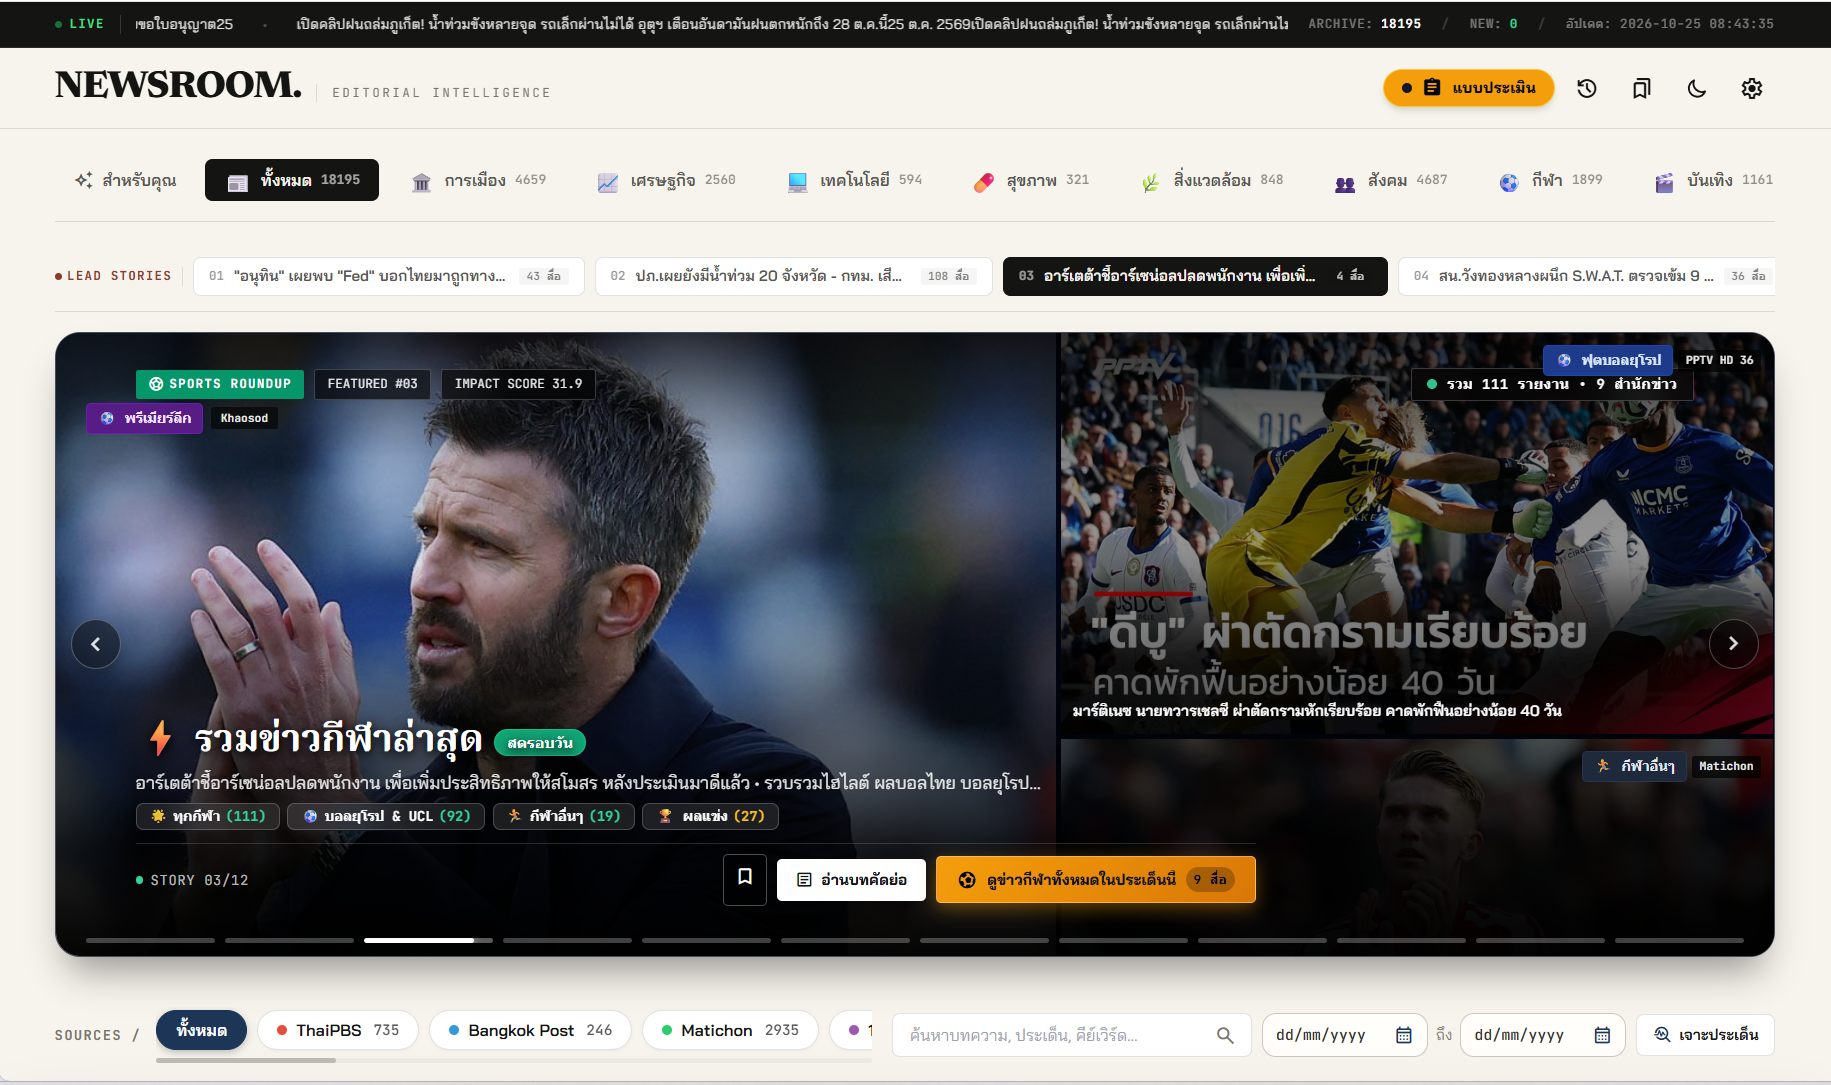
\includegraphics[width=0.95\textwidth]{images/screenshot_m01_bento_hub.png}}
\caption{หน้าจอหลัก Bento Hub SPA สำรวจข่าวสารสดประจำวัน}
\label{fig_screenshot_bento}
\end{figure}

\section{หน้าต่างพรีวิวเนื้อหาข่าวและบทสรุป In-App Reader}

หน้าต่างโมดอลสำหรับเปิดแสดงตัวอย่างเนื้อหาข่าวในตัวเว็บ (In-App Reader) ซึ่งได้รับการออกแบบตามหลักความสอดคล้องด้านการคุ้มครองลิขสิทธิ์ (Copyright Protection Compliance) โดยระบบจะไม่นำเนื้อหาบทความข่าวฉบับเต็มของสำนักข่าวต้นทางมาเปิดให้อ่านทั้งหมด แต่จะนำเสนอเฉพาะส่วนพรีวิวเนื้อหาบางส่วน ที่ผ่านการทำความสะอาดด้วย Trafilatura เพื่อตัดโฆษณา สคริปต์ และสิ่งรบกวน พร้อมปุ่มเชื่อมโยงเปิดอ่านบทความฉบับเต็มจากเว็บไซต์สำนักข่าวต้นทางโดยตรง สำหรับการกดปุ่มสรุปเนื้อหาด้วยปัญญาประดิษฐ์ (AI Summarization) ระบบฝั่งเซิร์ฟเวอร์จะนำเนื้อหาบทความฉบับเต็มทั้งหมด (Whole Article Content) มาทำการสังเคราะห์ (Synthesize) เพื่อสกัดสาระสำคัญ ประเด็นสำคัญ (Key Takeaways) และผลวิเคราะห์อารมณ์ของข่าวจากโมเดลภาษาขนาดใหญ่ได้อย่างครบถ้วนลึกซึ้ง พร้อมปุ่มบันทึกคั่นหน้าบทความ ดังแสดงในภาพที่~\ref{fig_screenshot_reader}

\begin{figure}[H]
\centering
\imgframe{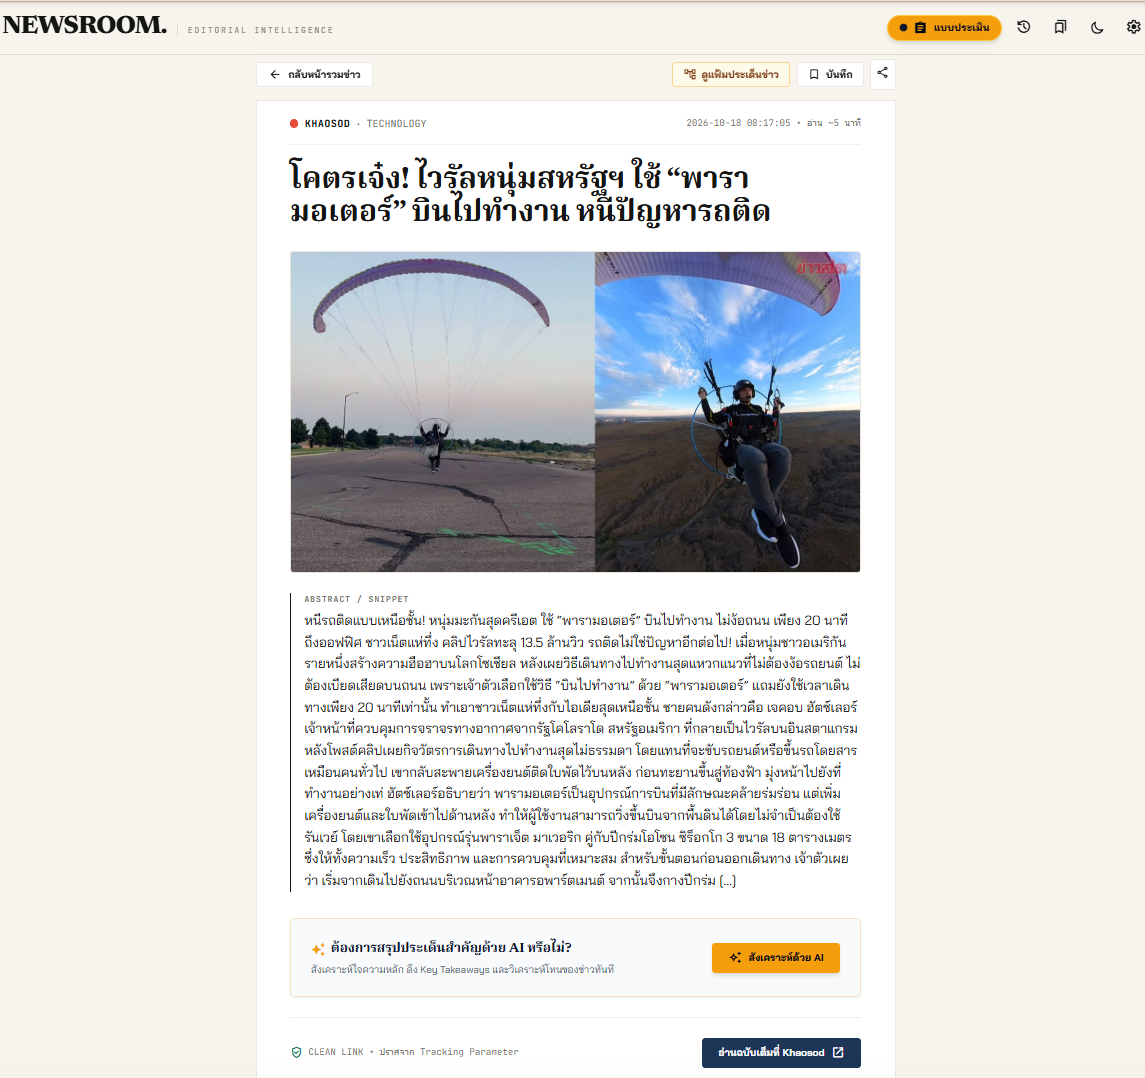
\includegraphics[width=0.95\textwidth]{images/screenshot_m02_in_app_reader.png}}
\caption{หน้าต่างพรีวิวเนื้อหาข่าว In-App Reader และปุ่มสังเคราะห์สรุปด้วย AI}
\label{fig_screenshot_reader}
\end{figure}

\section{แฟ้มเจาะลึกมหากาพย์ประเด็นข่าว Macro Storyline Dossier}

หน้าต่างแสดงผลแฟ้มเจาะลึกมหากาพย์ประเด็นข่าวที่เชื่อมโยงเหตุการณ์ย่อยเข้าด้วยกัน นำเสนอภาพรวมสถานการณ์ ไทม์ไลน์วิวัฒนาการของเหตุการณ์ตามลำดับเวลา และตารางข้อเท็จจริงที่ได้รับการยืนยันตรงกันข้ามสำนักข่าว (Corroborated Facts) พร้อมรหัสอ้างอิงรายประโยคไปยังบทความต้นทาง ดังแสดงในภาพที่~\ref{fig_screenshot_dossier}

\begin{figure}[H]
\centering
\imgframe{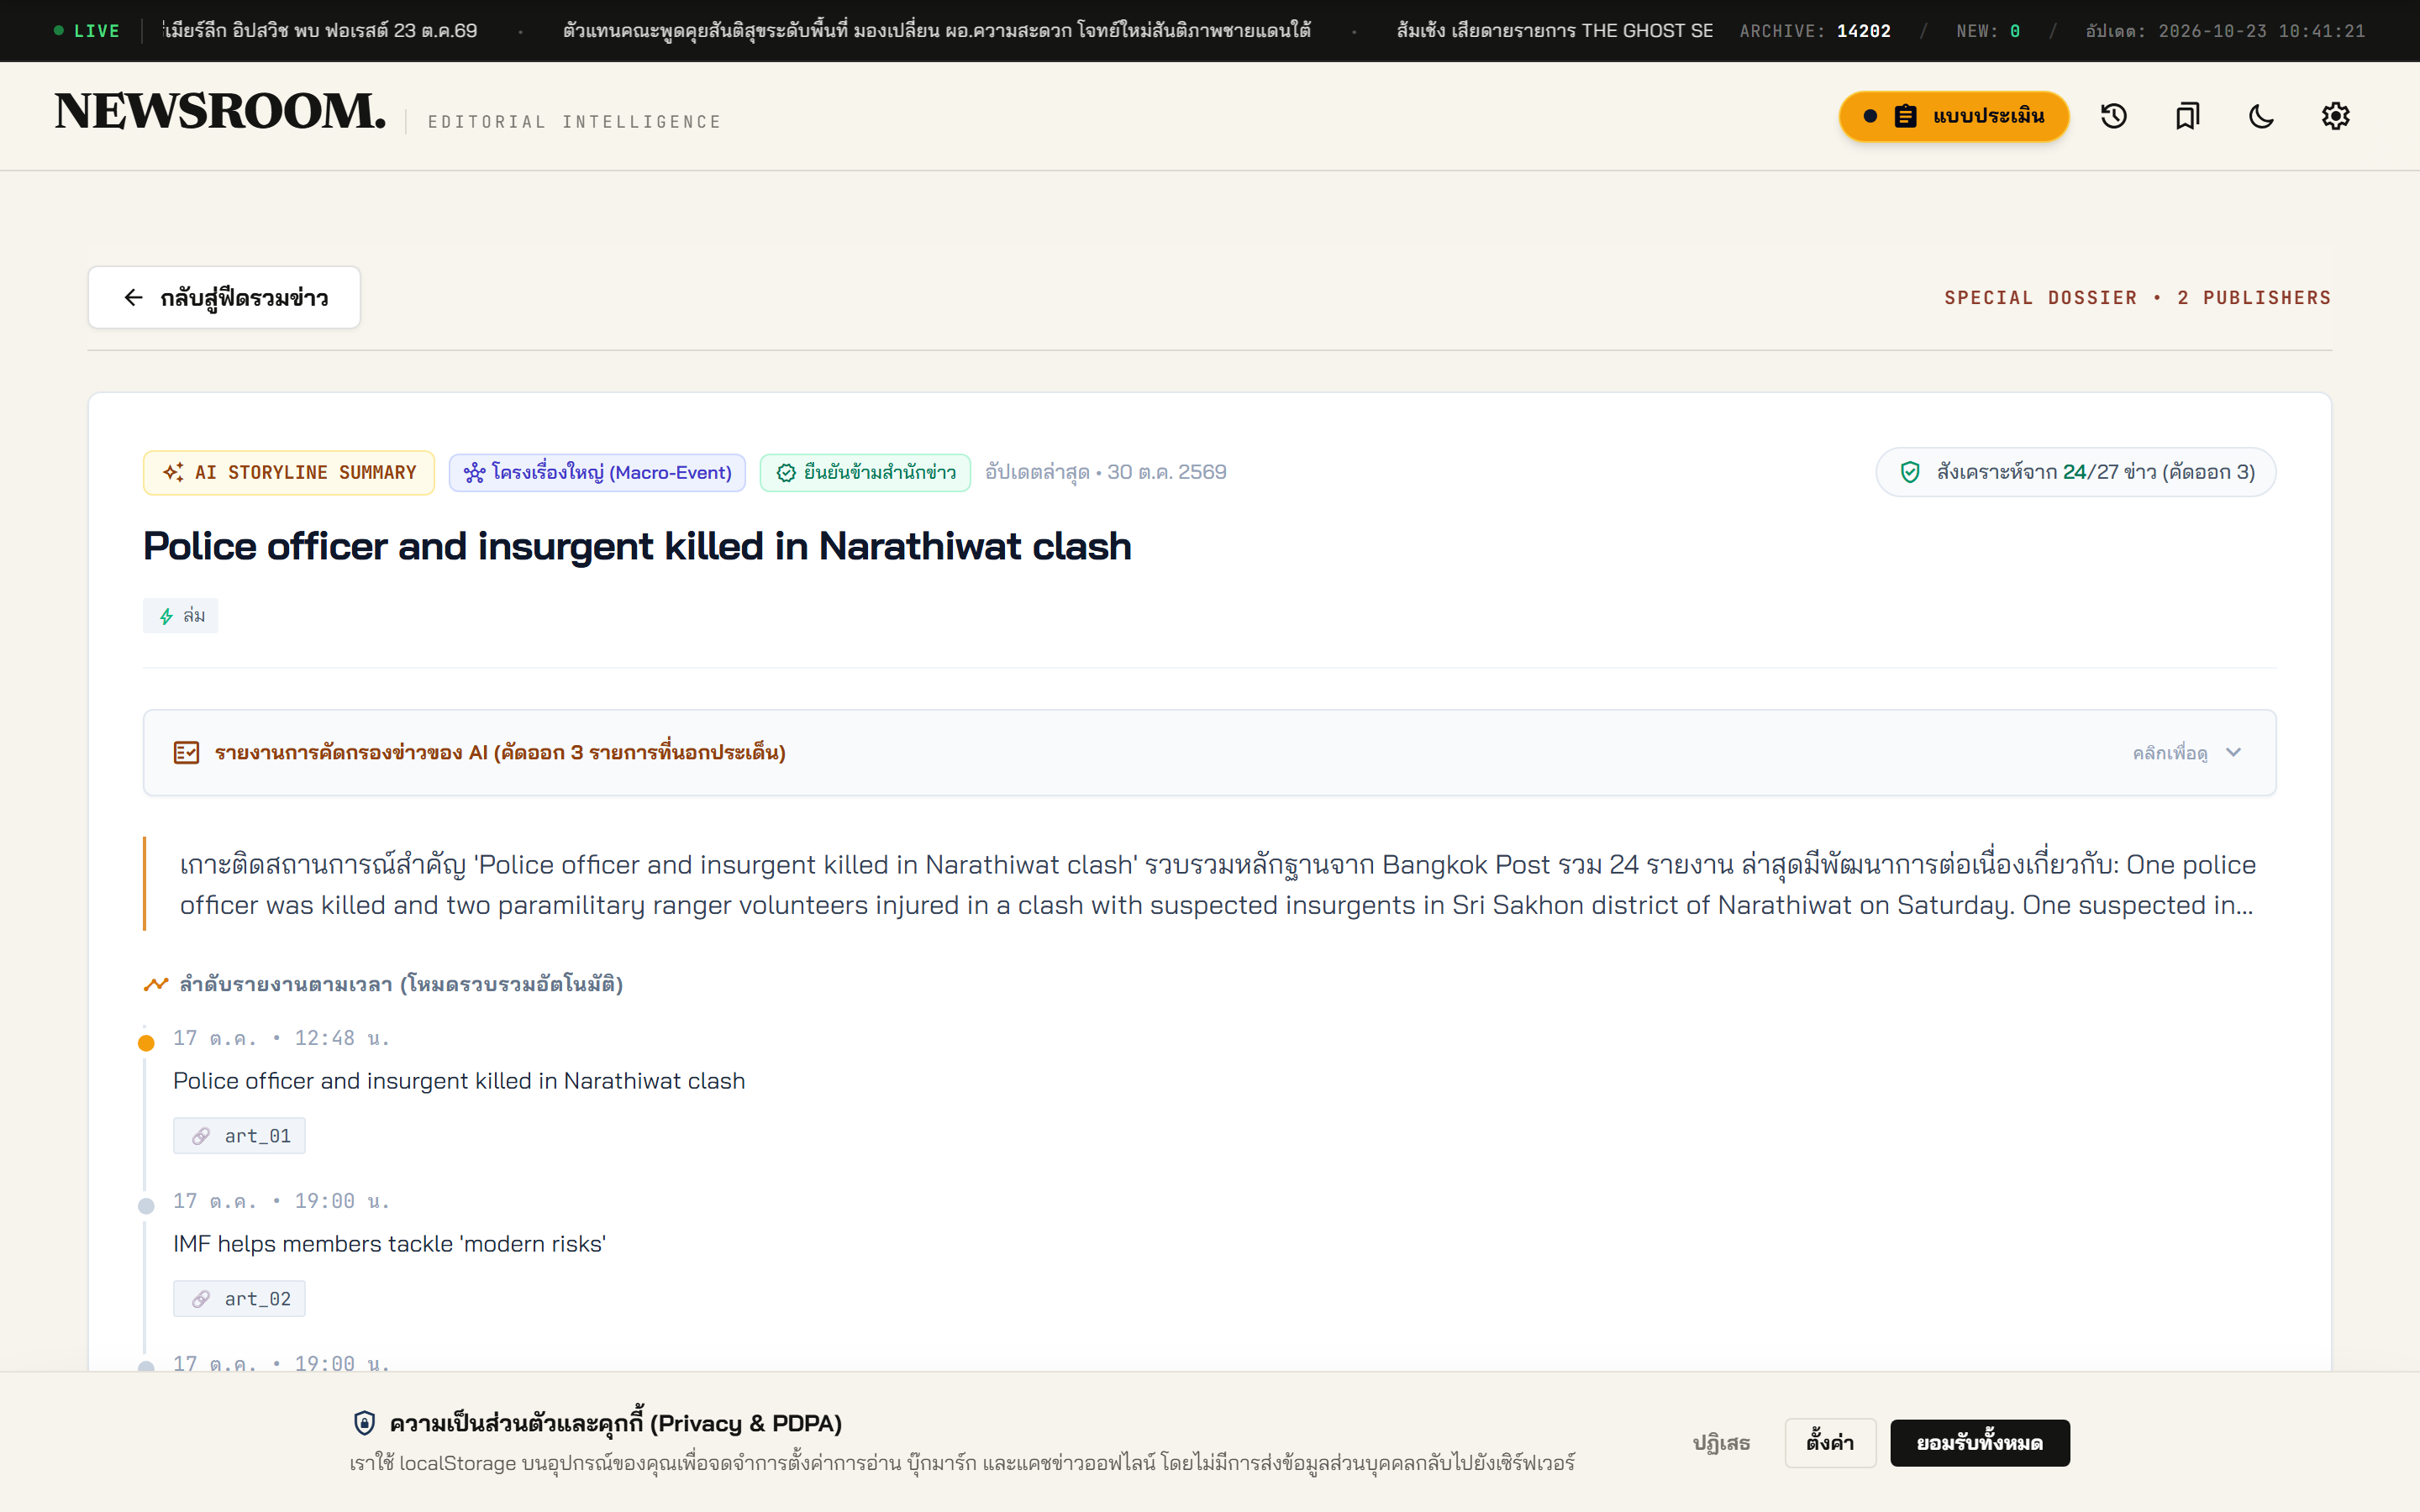
\includegraphics[width=0.95\textwidth]{images/screenshot_m03_macro_dossier.png}}
\caption{แฟ้มเจาะลึกมหากาพย์ประเด็นข่าวและไทม์ไลน์พัฒนาการเหตุการณ์}
\label{fig_screenshot_dossier}
\end{figure}

\section{สถานีเจาะประเด็นข่าวและสืบค้นเชิงวิเคราะห์ Issue Explorer}

หน้าต่างสถานีเจาะประเด็นข่าวเชิงวิเคราะห์ (Issue Explorer Workstation) สำหรับผู้อ่านและนักวิเคราะห์ข่าว รองรับการสืบค้นด้วยไวยากรณ์บูลีนขั้นสูง มีระบบขยายคำพ้องความหมายและคำย่อหน่วยงานรัฐ พร้อมแสดงการแจกแจงมุมมองของแต่ละสำนักข่าวและตัวกรองคัดแยกข่าวหลุดประเด็น ดังแสดงในภาพที่~\ref{fig_screenshot_explorer}

\begin{figure}[H]
\centering
\imgframe{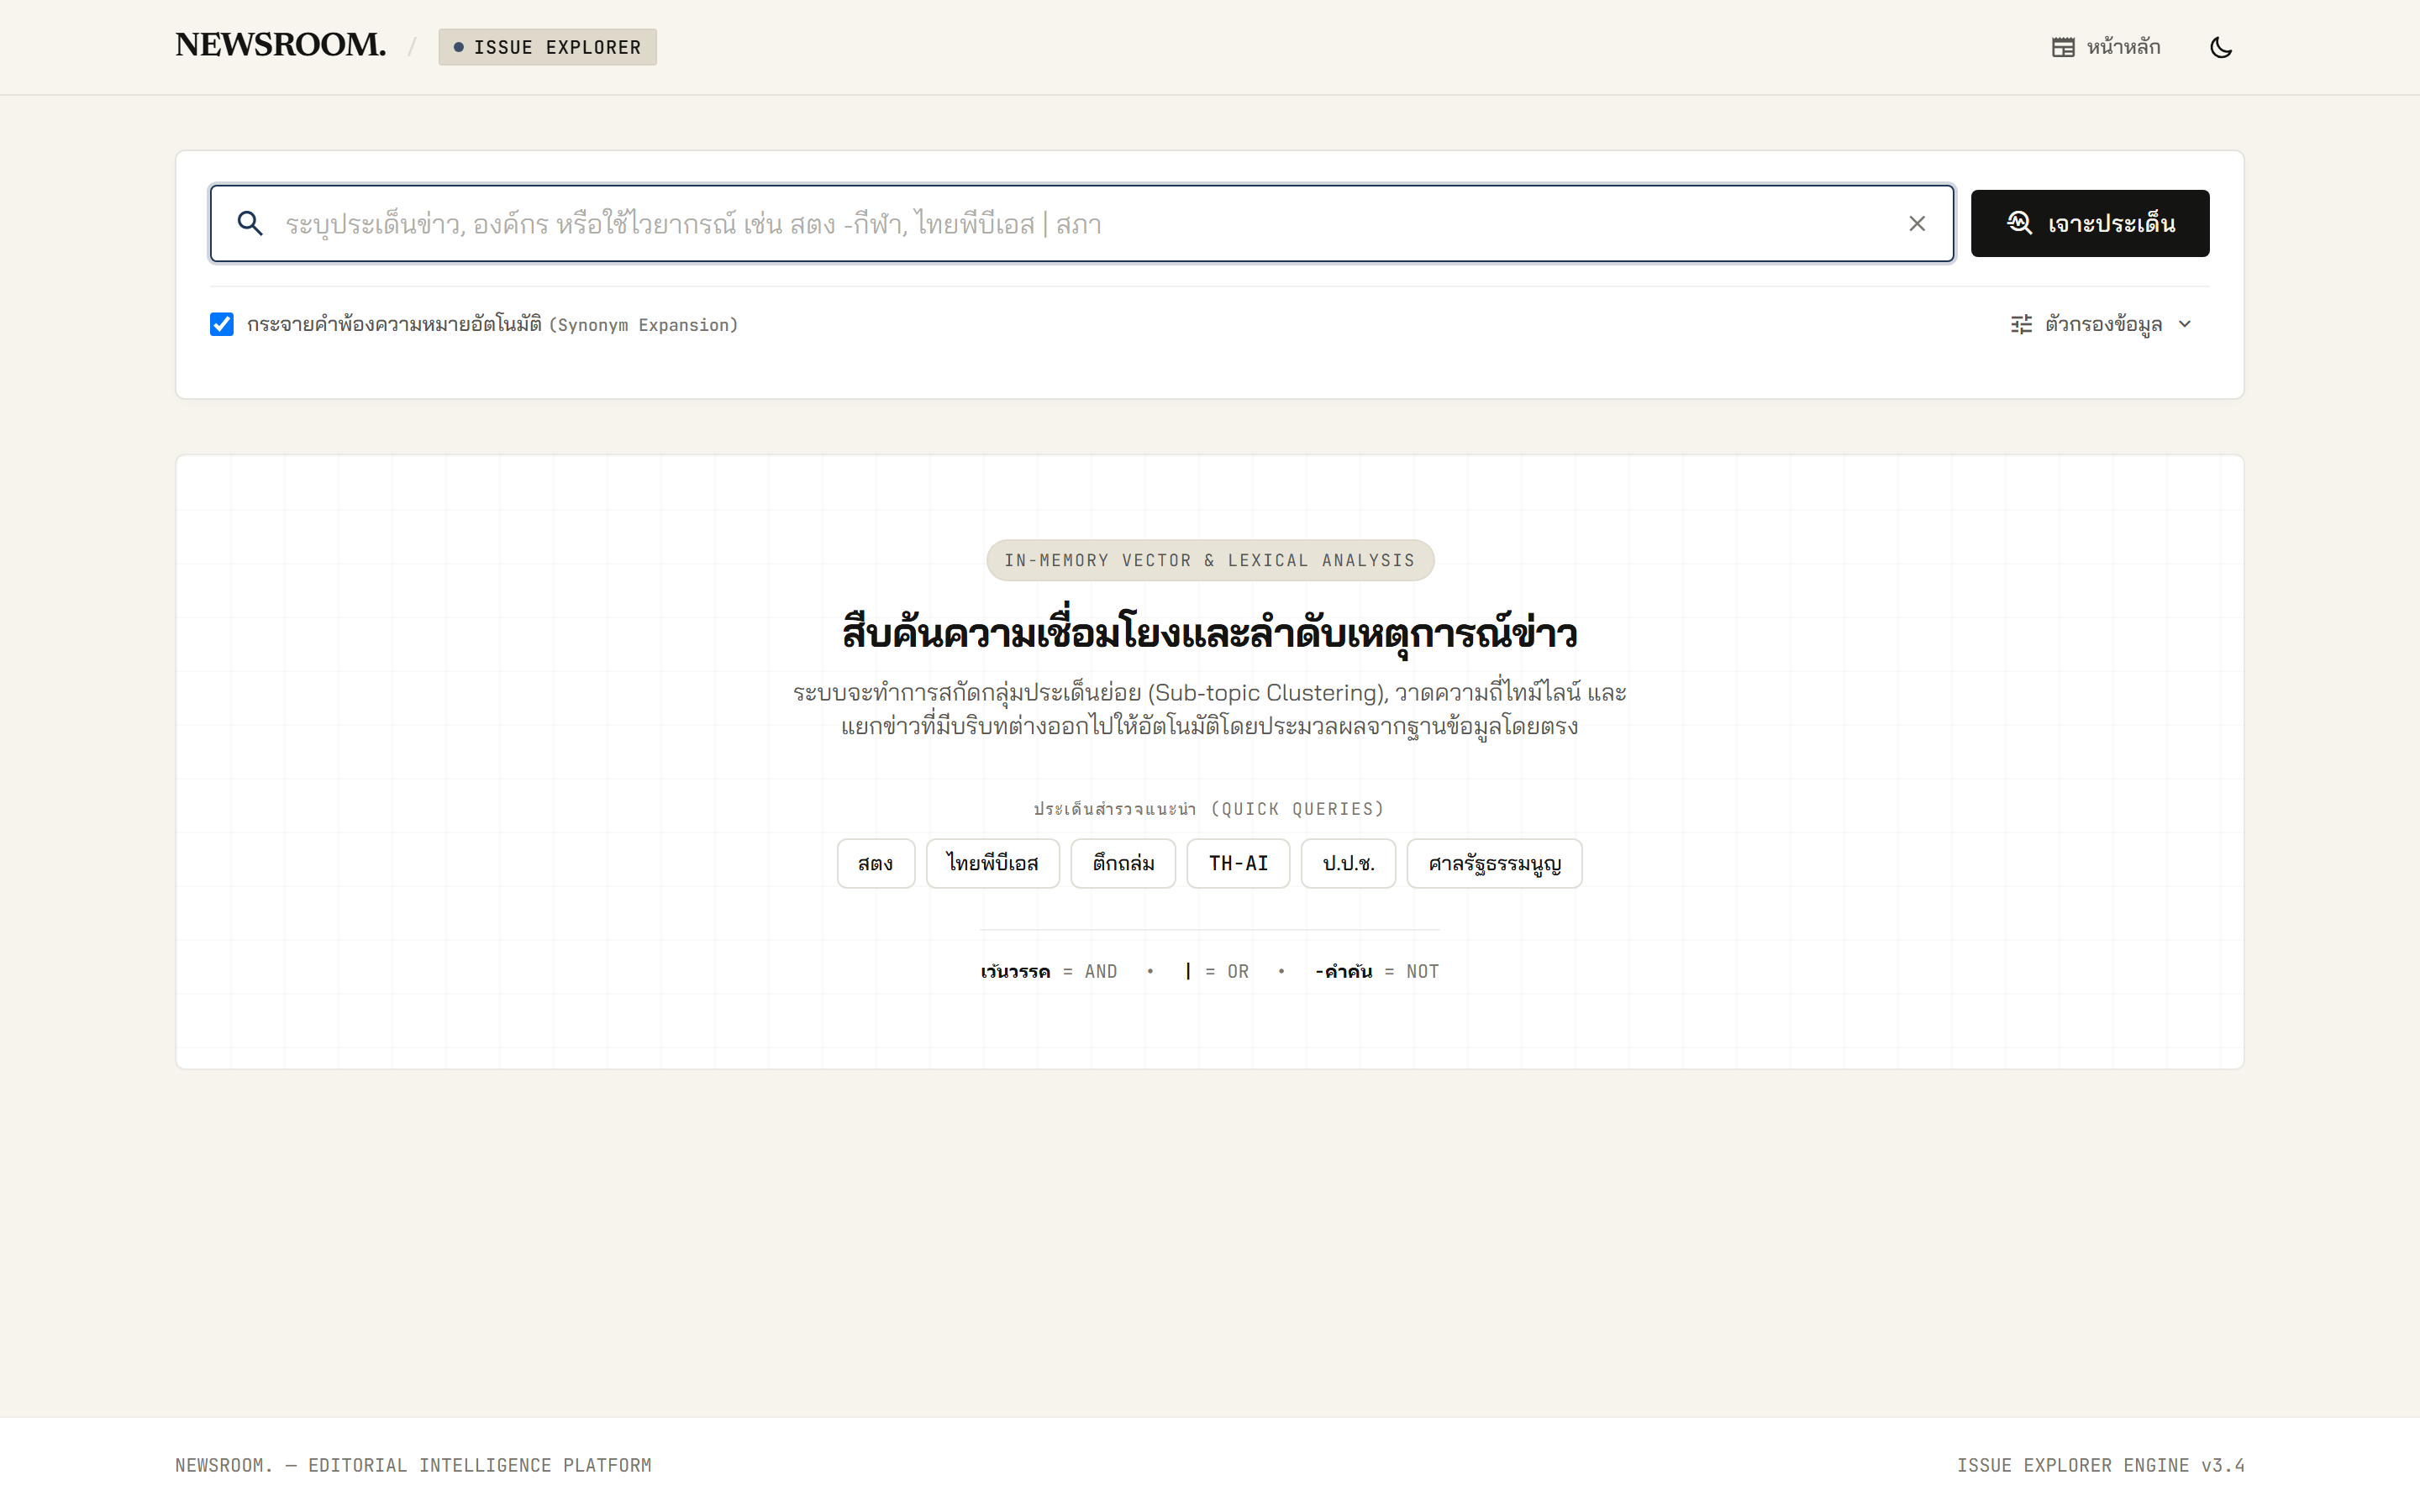
\includegraphics[width=0.95\textwidth]{images/screenshot_m04_issue_explorer.png}}
\caption{สถานีเจาะประเด็นข่าวและสืบค้นเชิงวิเคราะห์ Issue Explorer}
\label{fig_screenshot_explorer}
\end{figure}

เมื่อผู้ใช้งานพิมพ์คำสำคัญเพื่อค้นหาในสถานีเจาะประเด็นข่าว ระบบจะทำการสืบค้นข้อมูลเชิงลึกแบบทันที พร้อมทั้งแสดงผลลัพธ์รายการข่าวที่เกี่ยวข้อง การแจกแจงมุมมองเชิงเปรียบเทียบของแต่ละสำนักข่าว และตัวกรองคัดแยกประเด็นที่ตรงกับเงื่อนไขการค้นหา ดังแสดงในภาพที่~\ref{fig_screenshot_issue_output}

\begin{figure}[H]
\centering
\imgframe{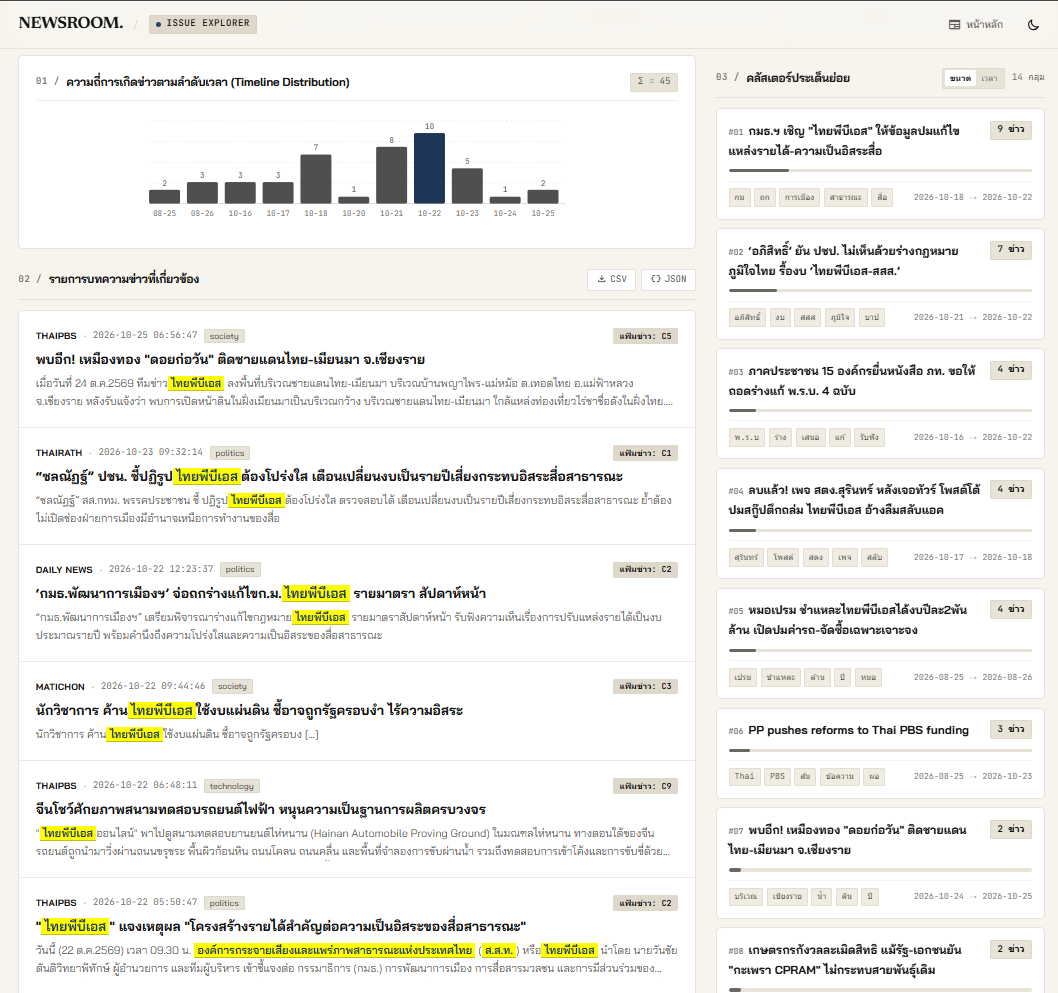
\includegraphics[width=0.95\textwidth]{images/issue_output.png}}
\caption{ผลลัพธ์การสืบค้นและคัดกรองประเด็นข่าวเชิงลึกบน Issue Explorer}
\label{fig_screenshot_issue_output}
\end{figure}

\section{ศูนย์ควบคุมและตรวจสอบสถานะระบบ Ops Monitoring Console}

หน้าต่างคอนโซลควบคุมการทำงานของระบบสำหรับผู้ดูแลระบบ แสดงสถานะความพร้อมของบริการ สถิติอัตรา Throughput การดึงข่าว ปริมาณการใช้หน่วยความจำ RAM สถานะการทำงานของแคช พร้อมปุ่มคำสั่งเริ่มสเกรปข่าวด่วนทันที ปุ่มคำสั่งล้างแคชในหน่วยความจำและแคช HTTP และเครื่องมือทดสอบการดึงข้อมูลรายสำนักข่าว ดังแสดงในภาพที่~\ref{fig_screenshot_ops}

\begin{figure}[H]
\centering
\imgframe{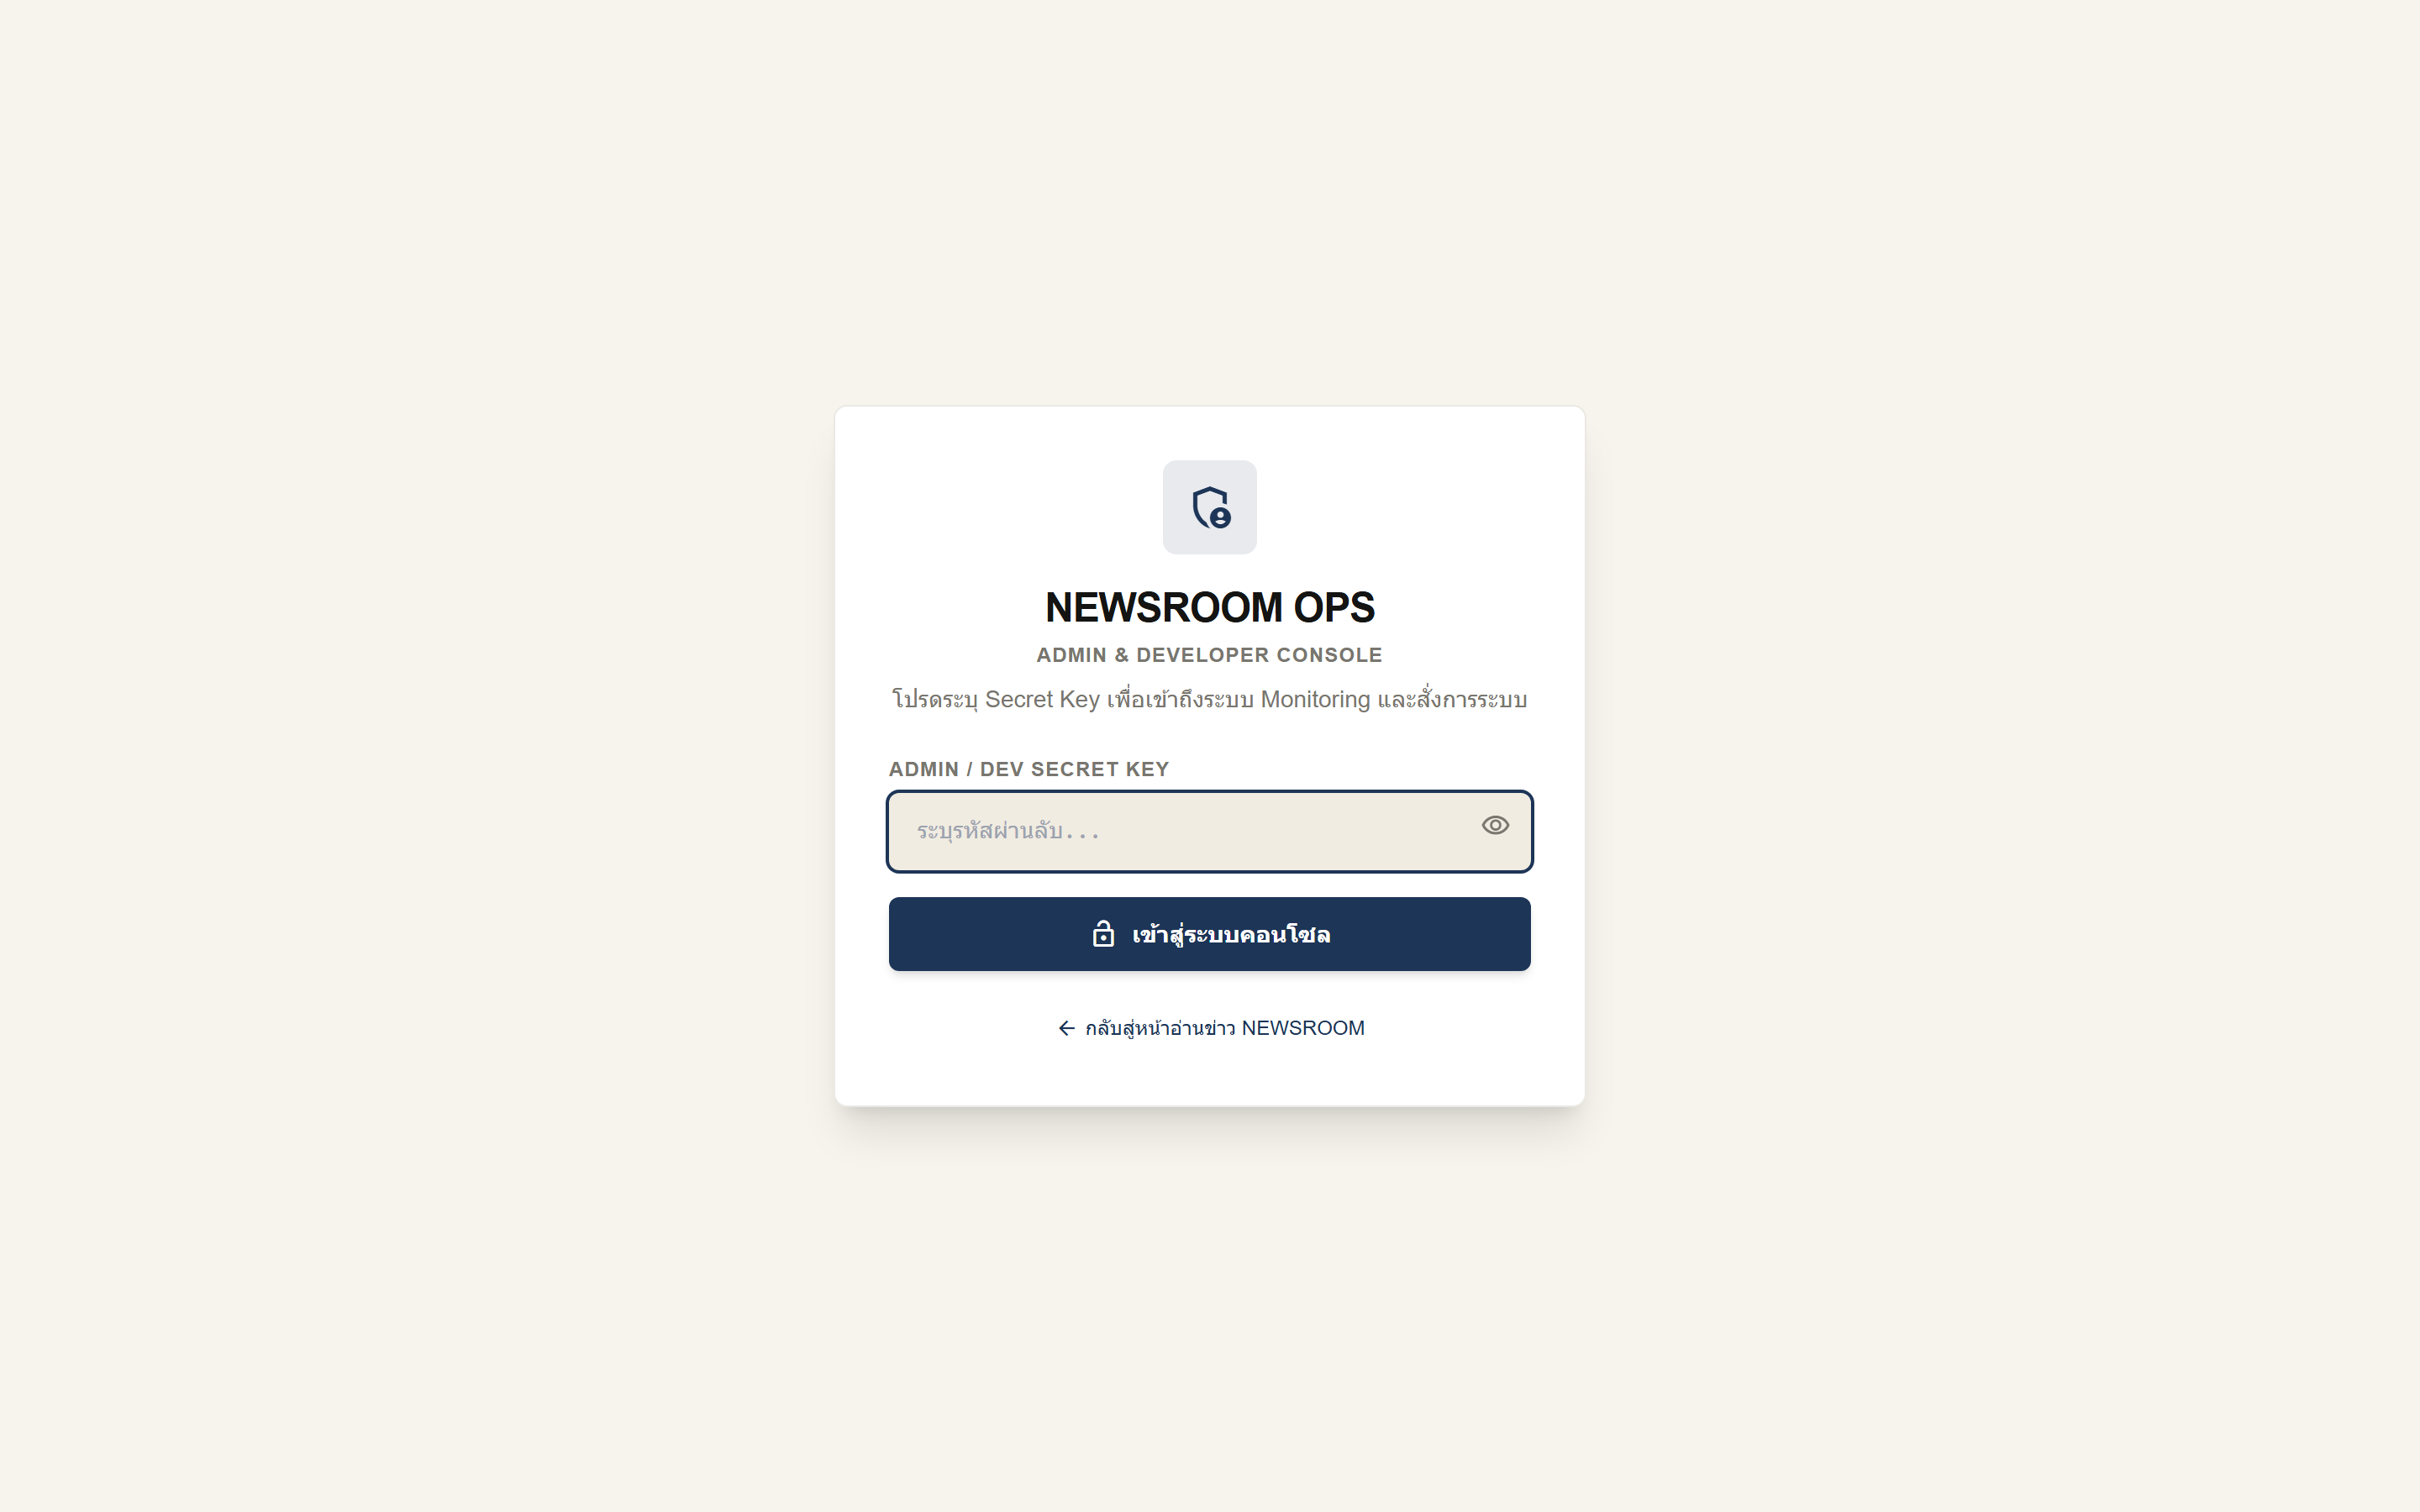
\includegraphics[width=0.95\textwidth]{images/screenshot_m05_ops_console.png}}
\caption{ศูนย์ควบคุมและตรวจสอบสถานะระบบ Ops Monitoring Console}
\label{fig_screenshot_ops}
\end{figure}

\section{หน้าต่างตั้งค่าสิทธิ์ความเป็นส่วนตัวและคุกกี้ Privacy Preferences}

หน้าต่างจัดการสิทธิ์ความเป็นส่วนตัวและการใช้คุกกี้ตามพระราชบัญญัติคุ้มครองข้อมูลส่วนบุคคล (PDPA) แสดงแถบขอความยินยอมคุกกี้ ตัวเลือกการเปิดหรือปิดใช้งานคุกกี้บันทึกความสนใจ และปุ่มสั่งล้างสถิติประวัติการอ่านออกจากหน่วยความจำของเว็บเบราว์เซอร์ได้ทันทีโดยสมบูรณ์ ดังแสดงในภาพที่~\ref{fig_screenshot_privacy}

\begin{figure}[H]
\centering
\imgframe{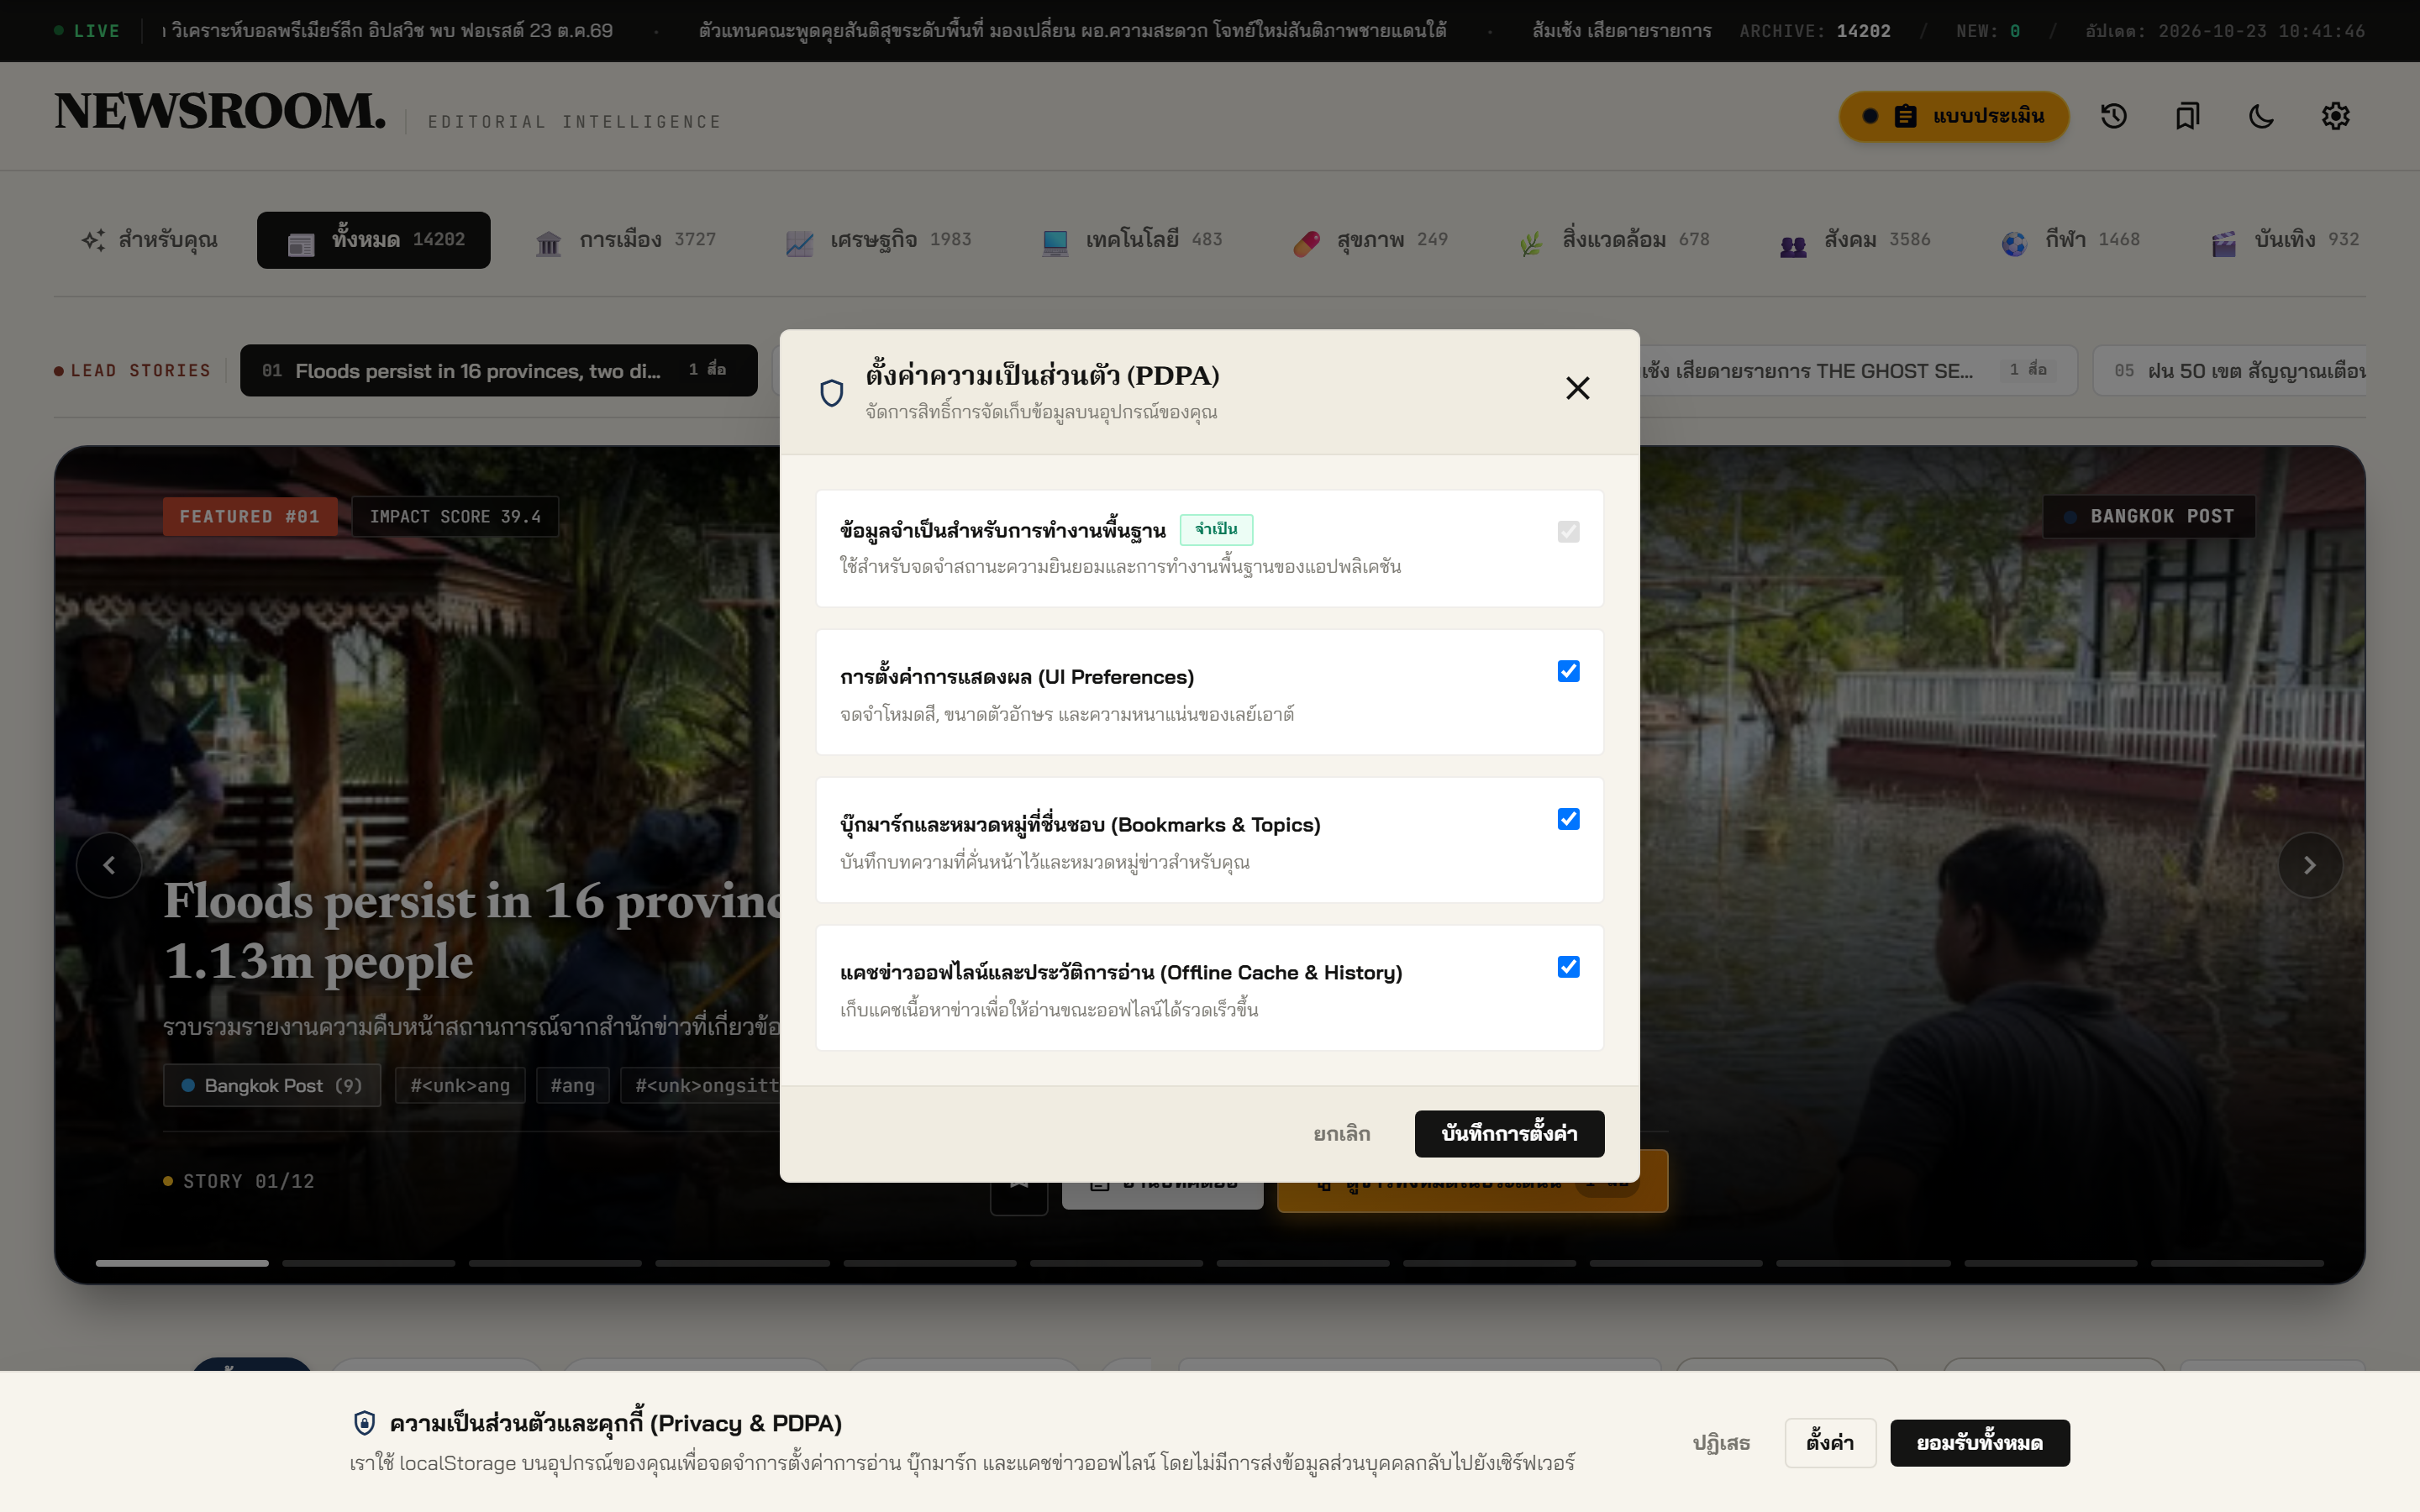
\includegraphics[width=0.95\textwidth]{images/screenshot_m06_privacy_modal.png}}
\caption{หน้าต่างตั้งค่าสิทธิ์ความเป็นส่วนตัวและคุกกี้ตามมาตรฐาน PDPA}
\label{fig_screenshot_privacy}
\end{figure}

\section{หน้าต่างปรับแต่งฟีดข่าวเฉพาะคุณ Personal Briefing}

หน้าต่างปรับแต่งฟีดข่าวเฉพาะบุคคล (Personal Briefing Onboarding) สำหรับผู้ใช้งานที่ต้องการสร้างฟีดข่าวตามความสนใจ โดยเปิดให้เลือกหมวดหมู่ที่สนใจอย่างน้อย 3 หมวดหมู่จากทั้งหมด 9 หมวดหมู่ พร้อมระบบจัดอันดับข่าวบนอุปกรณ์ของผู้ใช้งานโดยตรง (On-device Edge Personalization) ภายใต้มาตรฐานการคุ้มครองข้อมูลส่วนบุคคล (PDPA) โดยไม่มีการส่งประวัติการอ่านหรือข้อมูลส่วนตัวกลับไปยังเซิร์ฟเวอร์ ดังแสดงในภาพที่~\ref{fig_screenshot_feed_for_u}

\begin{figure}[H]
\centering
\imgframe{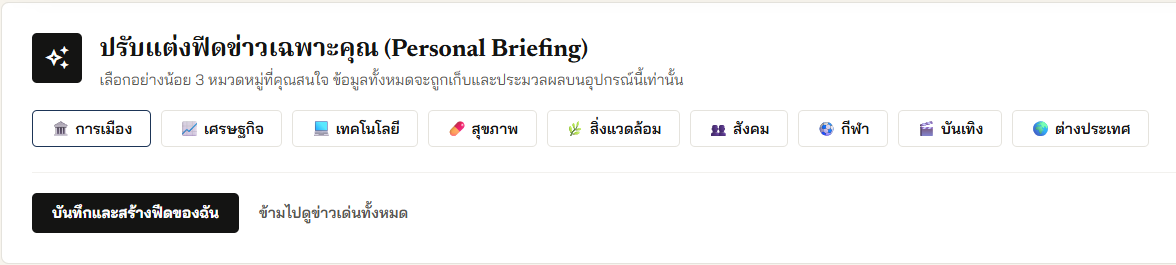
\includegraphics[width=0.95\textwidth]{images/feed_for_u.png}}
\caption{หน้าต่างปรับแต่งฟีดข่าวเฉพาะคุณสำหรับการสร้างฟีดตามความสนใจ}
\label{fig_screenshot_feed_for_u}
\end{figure}
